\documentclass[10pt,twocolumn,letterpaper]{article}

\usepackage{cvpr}
\usepackage{times}
\usepackage{epsfig}
\usepackage{graphicx}
\usepackage{amsmath}
\usepackage{amssymb}

% Include other packages here, before hyperref.

% If you comment hyperref and then uncomment it, you should delete
% egpaper.aux before re-running latex.  (Or just hit 'q' on the first latex
% run, let it finish, and you should be clear).
\usepackage[pagebackref=true,breaklinks=true,letterpaper=true,colorlinks,bookmarks=false]{hyperref}

% \cvprfinalcopy % *** Uncomment this line for the final submission

\def\cvprPaperID{2254} % *** Enter the CVPR Paper ID here
\def\httilde{\mbox{\tt\raisebox{-.5ex}{\symbol{126}}}}

% Pages are numbered in submission mode, and unnumbered in camera-ready
\ifcvprfinal\pagestyle{empty}\fi
\begin{document}

%%%%%%%%% TITLE
\title{Coupling Uncertain Active Constellation Models with \\
Cascaded Forest Predictors for Sematic Segmentation \\ -- Supplement --}

\author{First Author\\
Institution1\\
Institution1 address\\
{\tt\small firstauthor@i1.org}
% For a paper whose authors are all at the same institution,
% omit the following lines up until the closing ``}''.
% Additional authors and addresses can be added with ``\and'',
% just like the second author.
% To save space, use either the email address or home page, not both
\and
Second Author\\
Institution2\\
First line of institution2 address\\
{\tt\small secondauthor@i2.org}
}

\maketitle
%\thispagestyle{empty}

%%%%%%%%% ABSTRACT
%\begin{abstract}
We will include Figures~\ref{fig:var-importance}~and~\ref{fig:output-over-levels} of the supplementary material into the paper. 

%\end{abstract}
\section{Variable Importance}
%
\begin{figure*}[t]
\begin{center}
%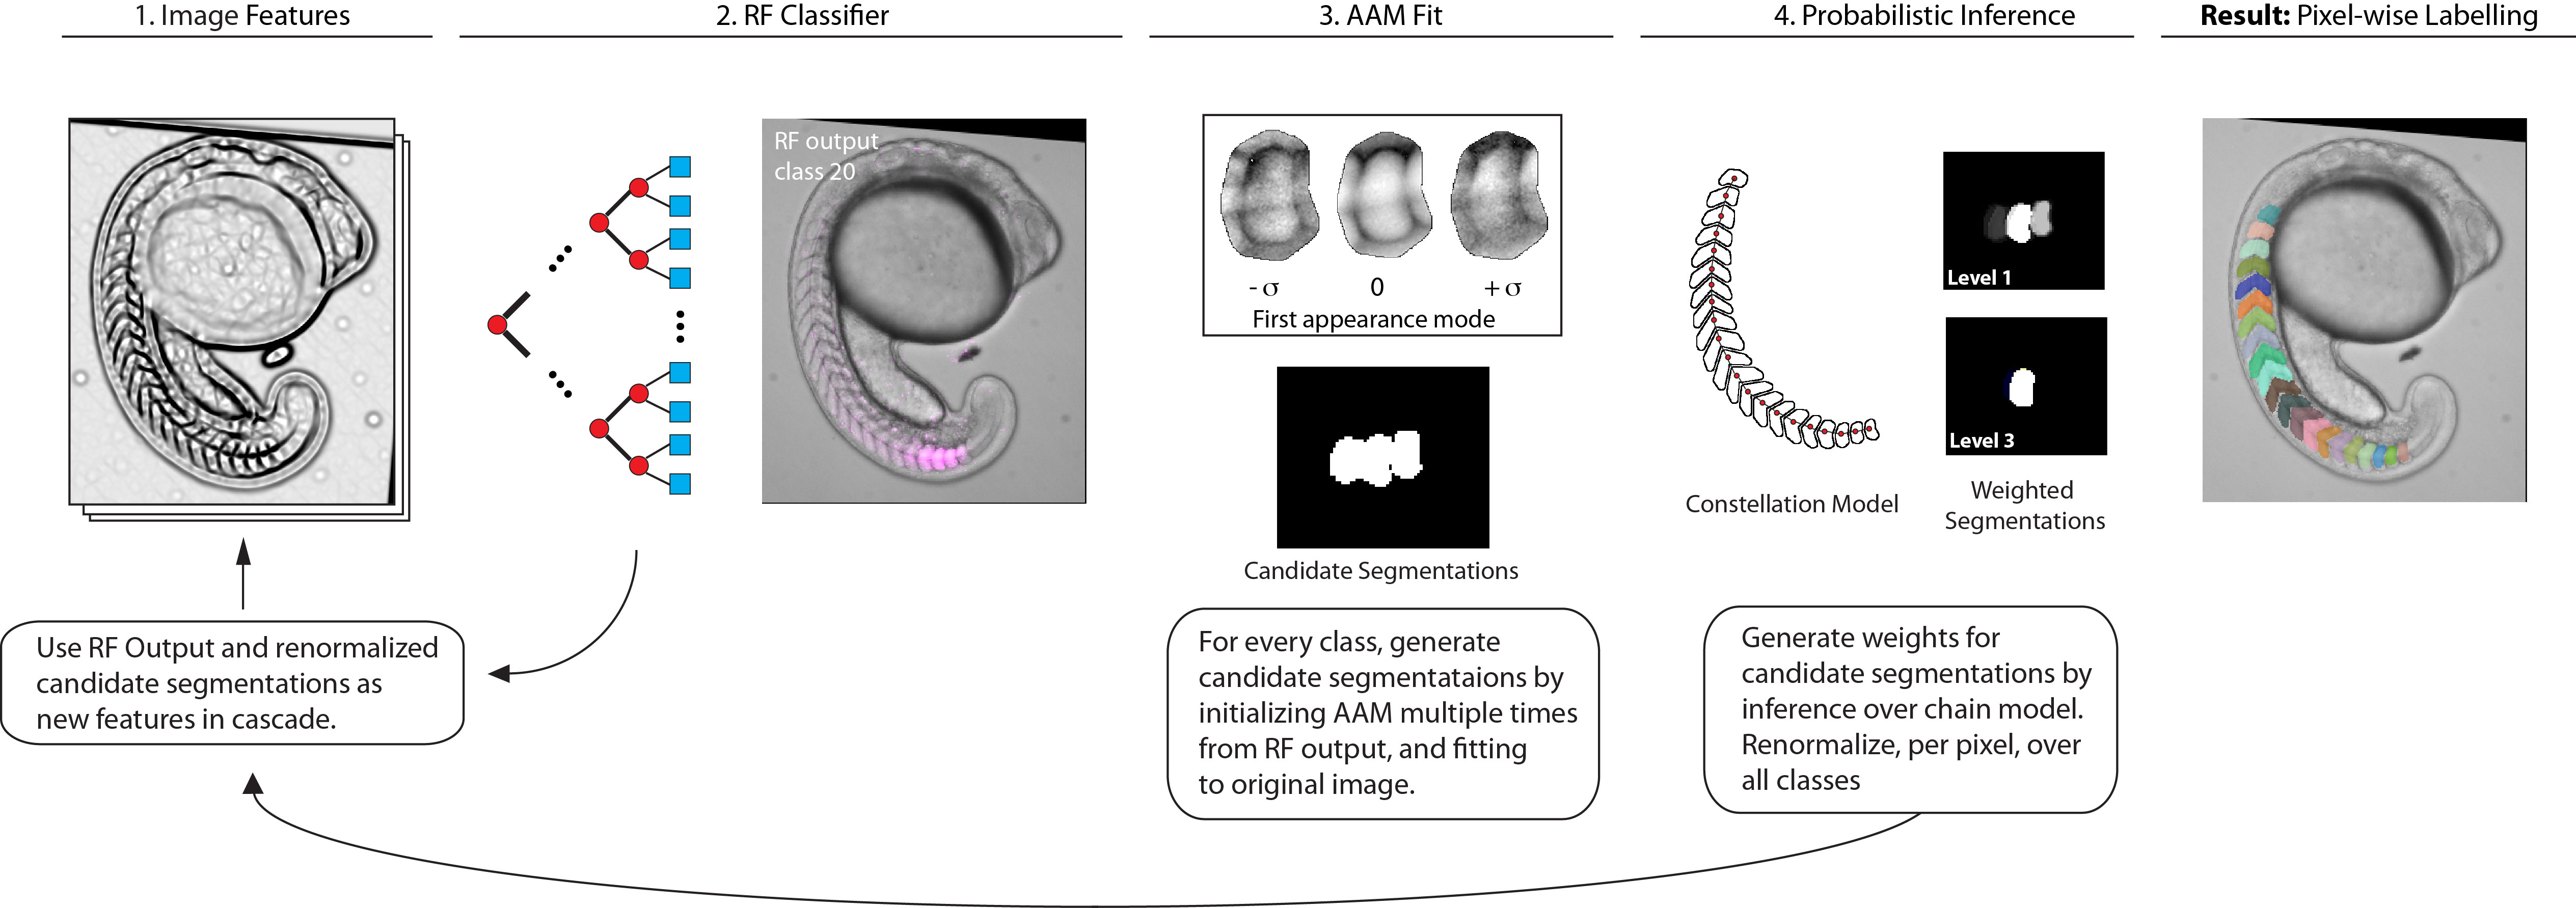
\includegraphics[width=\textwidth]{pipelineBIG2.jpg} 
\caption{We measure variable importance as defined in~\cite{BreimanRF}. Variable importance hints at how much worse the forest would perform (as a fraction of 1) without the respective feature. The tabel gives aggregated variable importance values for the filter bank features (1st column), the RF output (2nd column), and the smoothed RF output (3rd column). Top three rows: Our approach, three levels of the cascade. Bottom three rows: MAP instead of probabilistic inference. In the first level, only filter bank features are available. Hence the aggregated variable importance is 1 for the filter bank features, and zero otherwise. From the second level on variable importance reveals that smoothed RF output in the form of marginals is much more beneficial for the performance of the forest than the alternative MAP solution. }
\label{fig:var-importance}
\end{center}
\end{figure*}

\section{Additional Exemplary Results}
%
\begin{figure*}[t]
\begin{center}
%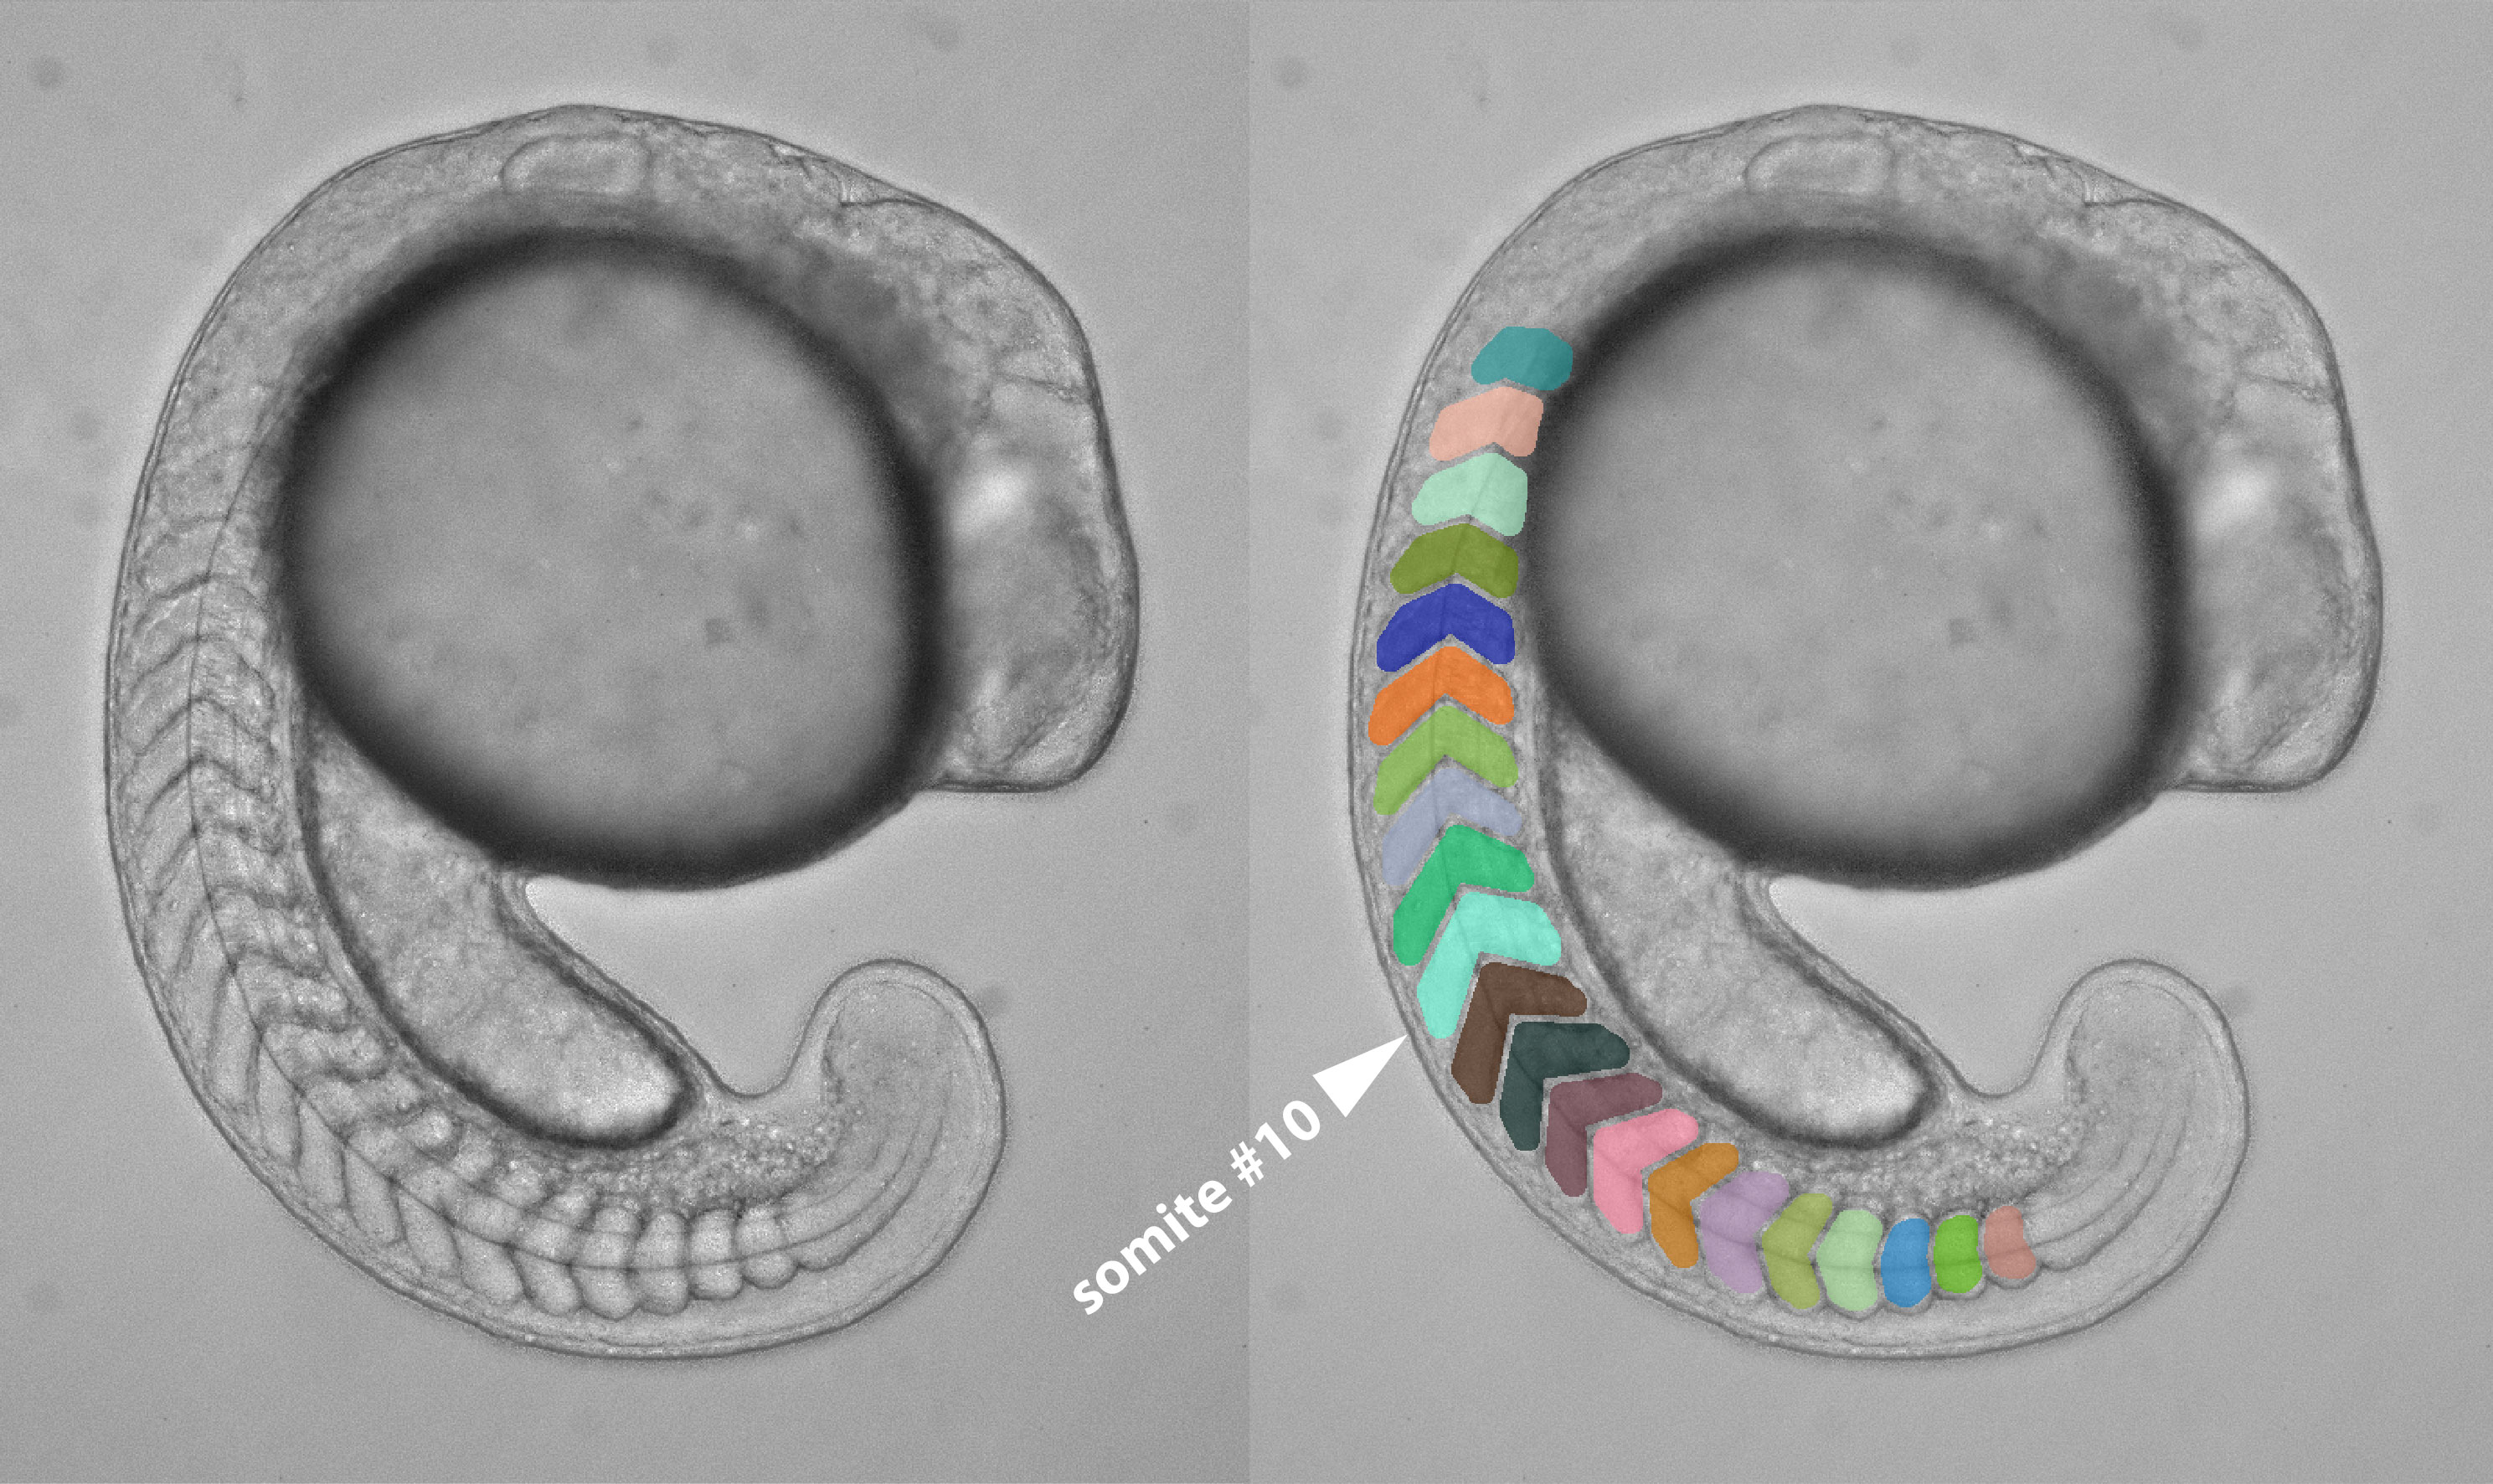
\includegraphics[width=\columnwidth]{TopRight.jpg} 
\caption{Output and smoothed output over levels }
\label{fig:output-over-levels}
\end{center}
\end{figure*}

{\small
\bibliographystyle{ieee}
\bibliography{somites2014-supplement}
}

\end{document}
